\documentclass[uplatex,dvipdfmx,a4j,openany]{jsarticle}
\input{"preamble.tex"}

\title{物質科学のための群論入門}
\author{ガオゾウ}

\begin{document}
\maketitle
\section{導入:物質の対称性と群論}
現実の物質を対象とする物質科学は、理論的な解析が非常に困難なことが多いです。その理由としては例えば、ほとんどの場合に自由度が非常に多いことや、相互作用を考慮しなくてはならないことが挙げられます。このような系では、理論的に厳密な解析をするのは困難であるため、しばしば大胆な近似を行う必要があります。

そんな物質の理論を構築するにあたり非常に重要となる一つの手がかりが、物質の持つ対称性です。対称性のもっとも簡単な例は「左右対称」でしょう。しばしば物質も「左右対称」を含む様々な対称性を持ちえます。実は、このような対称性を持つ・持たないという情報だけから物質の様々な性質を知ることができるのです。しかも、このような議論は、しばしば理論的に厳密に行うことができます。複雑な物質であっても、対称性は容易にわかることが多いので、これは非常に強力な手法です。

% 例えば、キラル分子が旋光性を持つ(光学活性である)というのは、まさに分子の持つ対称性から理解することができます。そのほか錯体分子の配位子場分裂や結晶場分裂は、その物質の持つ対称性の変化から生じるものです。
% また、固体物理学で最も基本的な理論であるバンド理論も物質の対称性に基づく理論の一つです。本来バンド理論は結晶中の電子の理論ですが、そこで出てくる「分散関係」という言葉がそのほかの様々な結晶中の粒子(フォノン、マグノン、etc.)にも用いられているのは、これらの理論は全て共通して結晶の持つ対称性を背景に持つからです。

% いろいろと例を挙げましたが、物理・化学と分野を問わず、物質科学において「対称性」が非常に基本的な考え方であることがわかっていただけたでしょうか。

このような対称性の議論をするにあたって基本的な道具となるのが、本記事のテーマである群論、特に群の表現論です。

本記事の基本的な流れは以下のようになります。まず、群の定義を簡単に述べた後、群の表現の定義を述べます。その後、群の表現に関する重要な定理をいくつか紹介します。その後、これらの定理を用いた実際の物質の解析例として、結晶場分裂を紹介します。

前提知識としては、線形代数と量子力学の基本的な知識を仮定します。「シュレーディンガー方程式を解くということはハミルトニアンを対角化することだ」と言われて意味がわかれば大丈夫です。群論については、一応群の公理から話を始めるので、前提知識は原理的にはいりません。しかし、多少は触れたことがあった方が話は分かりやすいとは思います。

本記事ではあくまで物質の解析への応用を主眼とするので、定理の証明にはあまり踏み込みません。興味のある方は参考文献にも挙げている応用群論\cite{ouyougunron}などをご覧ください。また、本記事では有限群のみを扱います。本記事で群はすべて有限群を指すと思ってください。

%  対称性のもっとも簡単な例の一つは正方形です。正方形は様々な対称性を持っています。例えば、正方形は図1(a)のように、中心線に関して折りたたむときれいに重なります。つまり左右対称です。このことは、

 

% また、図1(b)のように90°(1/4回転)だけ正方形を回転しても、元の形に戻ります。このような対称性を4回対称性と呼びます。正方形は同時に、2回対称性も持ちます。すなわち、180°(1/2回転)だけの回転に対しても、やはり元の形に戻ります。

\section{対称性と群論の概観}
\subsection{群の定義}
群とは、以下の四つの公理を満たす集合$G$と演算$\vdot$(積と呼ぶ)の組$(G, \vdot)$のことを指します。
\begin{tcolorbox}[title = 群の公理]
	\begin{enumerate}
		\item $G$は積に関して閉じている。すなわち、任意の元$g, h \in G$に対して、$g\vdot h\in G$が成り立つ。
		\item 積に関して結合律が成り立つ。すなわち、任意の元$g_1, g_2, g_3 \in G$に対して、\begin{align}
			g_1 \vdot (g_2 \vdot g_3) = (g_1 \vdot g_2) \vdot g_3
		\end{align}
		が成り立つ。
		\item $G$は単位元$e$を持つ。すなわち、任意の元$g\in G$に対し$g\vdot e = e\vdot g = g$となるような元$e\in G$が存在する。
		\item 任意の$G$の元に対し、積に関する逆元が存在する。すなわち、任意の元$g\in G$に対し、ある$g'\in G$が存在し、\begin{align}
			g \vdot g' = g' \vdot g = e
		\end{align}が成り立つ。(このときの$g$に対する$g'$のことを$g^{-1}$とかく。)
	\end{enumerate}	
\end{tcolorbox}

ここで、一般に積に関して可換であるとは限らないことに注意してください。

群の例としてよく挙げられるのは、実数全体の集合$\mathbb{R}$と和$+$の組$(\mathbb{R}, +)$です。この場合単位元は0で、$a\in \mathbb{R}$に対する逆元は$-a$です。なお、実数は積に関しては群になりません。0に対する逆元が存在しないからです。

また、複素数係数のn次正則行列全体の集合$GL_n(\mathbb{C})$も、通常の行列積に関して群を成します。この場合の単位元は単位行列であり、逆元は逆行列になります(正則行列に対しては必ず逆行列が存在します)。

気分としては、逆元を持つような最低限「まとも」な演算を持つ集合のことを群と呼ぶ、と思っておけばとりあえずはよいと思います。

以下本記事では、誤解の恐れがない限り、積の記号$\vdot$は省略し、$g_1\vdot g_2$のことを単に$g_1g_2$と書きます。

\subsection{対称性の定式化と群}
さて、前節で定義した群はどのように物質における対称性の議論に用いられるのでしょうか。それを考えるためには、まず「対称性」という概念を数学的に定式化する必要があります。結論から言えば、対称性とは、ある変換に対して不変であることとして定式化されます。

\subsubsection{対称性と変換}
系がある変換に対して不変であるとき、その系は(その操作に対応する)対称性を持つと言われます。たとえば、簡単な場合として正方形を考えてみましょう。正方形は左右対称です。つまり、適当な中心線に対して正方形を折り返した時にピッタリ正方形が重なります(図\ref{fig:square_symmetry}(a))。このことは、正方形の中心に原点をとり、辺に平行に$x,y$軸をとったとき(図\ref{fig:square_coordinate})、正方形は$\sigma_x:x\mapsto -x$という変換$\sigma_x$に対して不変である、ということもできます。同様に、正方形は$\sigma_y:y\mapsto -y$という変換$\sigma_y$に対しても不変です。これは正方形が上下対称であるということに対応します。

\begin{figure}[htbp]
	\centering
	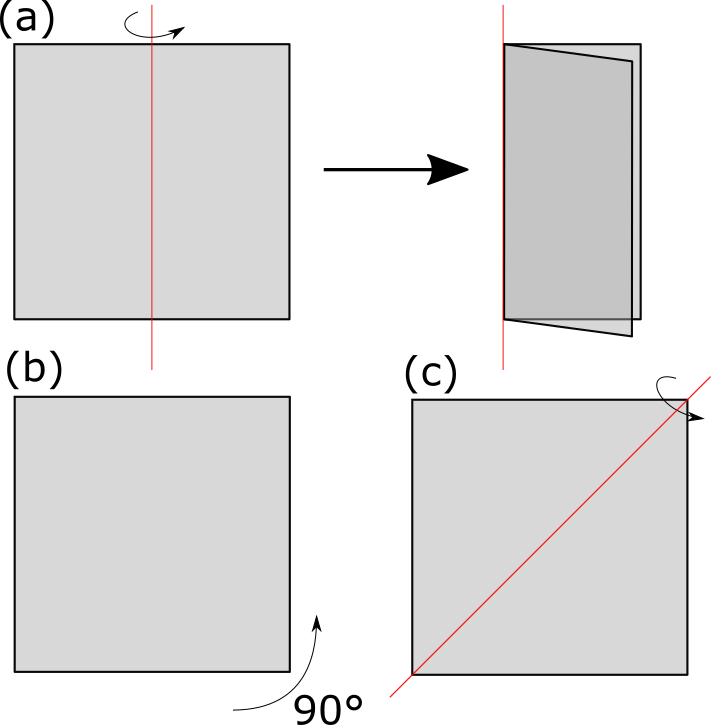
\includegraphics[width=0.7\columnwidth]{square_symmetry.png}
	\caption{正方形の対称性}
	\label{fig:square_symmetry}
\end{figure}

\begin{figure}[htbp]
	\centering
	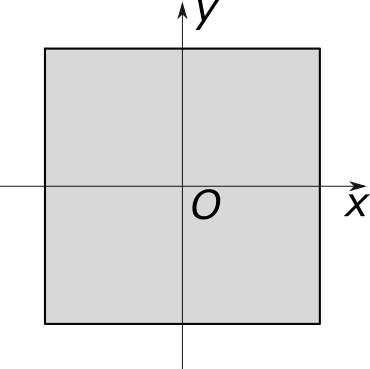
\includegraphics[width=0.4\columnwidth]{square_coordinate.png}
	\caption{正方形の座標系}
	\label{fig:square_coordinate}
\end{figure}

その他にも様々な対称性を、このような「ある変換に対する不変性」という形で定式化することができます。例えば、図\ref{fig:square_symmetry}(b),(c)はそれぞれ、正方形が90°回転、斜め方向の折り返しに関して不変である様子を表しています。これらも、それぞれ次のような変換に対応していると考えることができます。
\begin{align}
	C_4&: (x,y)\mapsto (-y,x)\\
	\sigma_d&: (x,y) \mapsto (y,x)
\end{align}

これらの変換はよく見るとすべて線形変換なので、行列を用いて表すことができます。例えば、
\begin{align}
	\sigma_x &= \mqty(-1 & 0 \\
					   0 & 1 ) \\
	C_4 &= \mqty(0 & -1 \\
				 1 & 0 )\\
	\sigma_d &= \mqty(0 & 1 \\
					1 & 0) \\
	\sigma_d' &= \mqty(0 & -1 \\
					  -1 & 0)
\end{align}
などです。これらの変換はすべて長さ(ノルム)を変えない直交変換になっていることにも注意してください。

さて、二つの変換を続けて行うことを、新しい一つの変換とみなせば、変換の合成を定義することができます。例えば、最初に$\sigma_x$という変換を行ってから、次に$C_4$という変換を行うことを$C_4 \circ \sigma_x$と書くことにしましょう。$C_4\circ \sigma_x$は、もちろん正方形を不変に保つ変換になっています。実際、先ほど導入した行列を用いて計算してみると、
\begin{align}
	C_4\circ \sigma_x &= 
	\mqty(	0	& -1 \\
		  	1	& 0 )
	\mqty(	-1	& 0 \\
			0	& 1 ) = 
	\mqty(	0	& -1 \\
			-1	& 0 ) = \sigma_d'
\end{align}
となっていて、合成した結果もまた正方形を不変にする変換の一つになっていることが確かめられます。他にも、例えば$\sigma_y\circ\sigma_y$は、
\begin{align}
	\sigma_y\circ\sigma_y &= 
	\mqty(	1	& 0 \\
			0	& -1 ) 
	\mqty(	1	& 0 \\
			0	& -1 ) = \mqty(\imat{2}) 		 
\end{align}
と、単位行列になることがわかります。単位行列は、何もしない変換ですから、当然正方形は不変にする変換の一つということができます。一般に、このような何もしない変換のことを恒等変換と呼び、本記事では$E$と書くことにします。

ここまでに述べたことをまとめます。本節では正方形を例にとって、系を不変にする変換について考えました。このとき、変換の合成や、恒等変換を考えることができました。勘のいいひとは気づいているかもしれませんが、これらの正方形を不変にする変換全体の集合は、変換の合成を積として群をなします。これこそが、本記事で考えたい「対称性を表す群」です。

より一般に、ある注目する系について、本節で述べたような系を不変にする変換をすべて集めてきた集合$G$を考えましょう。この集合は、変換の合成を積とみれば群になっています。この場合の単位元は、恒等変換$E$になります\footnote{このあたりの「何を対称性の群の定義にするか」という話については、正直自分もよくわからないが、フォーマルには後述の「ハミルトニアンを不変にする変換全体の集合」というのが最も良いと思う。このように考えればきちんとこの集合が群になっていることも示すことができる。ただ、実際にモデルを作ったりするときは、始めに対称性の群がありきで、その対称性を持つようなハミルトニアンを考えたりする。まあ物理なので細かいことは気にしない。}。


\subsubsection{量子力学における対称性と保存則} \label{sec:symmetry_in_qm}
前節では、正方形を例にとって対称性が変換に対する不変性という形でとらえられることを説明しました。また、系が不変になるような変換全体の集合が群になることを述べました。

ここでは、量子力学においてこのような変換がどのように表されるかということと、量子系の対称性から導かれる保存則について簡単に述べます。

量子力学において、対称性$g$に対応する変換はユニタリ変換$U_g$で表されます\footnote{時間反転対称性は反ユニタリ変換。}。このとき、ある状態$\ket{\psi}$は次のように変換されます:
\begin{align}
	\ket{\psi} \mapsto U_g\ket{\psi}
\end{align}
このとき、物理量$A$の期待値は次のように変化します。
\begin{align}
	\expval{A} = \expval{A}{\psi} \mapsto \expval{U_g^{\dagger}AU_g}{\psi}
\end{align}

この後、しばしば状態そのものではなく物理量に着目して調べていくことが多くなります。そこで、$g$による変換を状態ではなく物理量に押し付けて定式化することにしましょう。すなわち、状態ベクトル$\ket{\psi}$が$g$によって変換すると考えるのではなく、物理量の演算子$A$が$g$によって変換を受けると考えます。このように考えると、演算子$A$は次のように変換するのが自然であるとわかります:
\begin{align}
	A \mapsto U^{\dagger} A U
\end{align}

これを用いて量子系の対称性をキチンと定義しましょう。量子系は、あるハミルトニアン$H$によって記述されます。量子系がある対称性を持つということは、対称性$g$に対応するユニタリ変換$U_g$に対して、ハミルトニアンが不変であること、すなわち、
\begin{align}
	H = U_g^{\dagger} H U_g \qq{あるいは}	U_gH = HU_g \label{eq:commutator}
\end{align}
が成り立つこととして定義されます\footnote{この定義から、量子系の対称性に対応するユニタリ変換全体の集合は、確かに群をなしていることがわかります。}。

ところで、ハミルトニアンが対称性を持つとき、すなわち式\eqref{eq:commutator}が成り立つとき、ユニタリ変換$U_g$とハミルトニアンの固有状態$\ket{\psi}$の関係はどうなっているのでしょうか。直観的には、$\ket{\psi}$を$U_g$によって変換しても、ハミルトニアンが対応する不変性を持っているのであれば、エネルギー固有値は変わらないように思えます。これは実際正しいことが次のように確かめられます。
\begin{align}
	H\qty(U_g\ket{\psi}) &= U_gH\ket{\psi} = EU_g\ket{\psi}
\end{align}
ここで$E$は$\ket{\psi}$のエネルギー固有値です。したがって、$U_g\ket{\psi}$は$\ket{\psi}$と同じエネルギーを持つ状態であることがわかりました。$U_g\ket{\psi}$と$\ket{\psi}$は同じエネルギーを持ちますが、必ずしも量子力学的に同じ状態とは限らないことに注意してください。また、量子力学的に同じ状態であったとしても、位相因子分だけ異なっている可能性もあります。これらは「対称性$g$による変換$U_g$は、異なるエネルギー固有状態を混ぜることはない。すなわち、演算子$U_g$はエネルギー固有空間ごとにブロック対角化されている」と言い換えることもできます。

さて、ある一つの固有エネルギーに着目し、その固有空間だけを考えることにしましょう。すると、$U_g$はこの固有空間内だけで閉じたユニタリ変換になっています。しかも、このことは対称性の群$G$のすべての元$g$について成り立っています。
ここで、次のような問題を考えることができます:「このとき、どのような$U_g$や固有空間が許されるのか?」
つまり、「固有空間内だけで$U_g$の変換が閉じている」という事実そのものを、ハミルトニアンやエネルギー固有値に対する制約とみるのです。実は、群$G$に対して対応する$U_g$や固有空間は、(基底の取り方による自由度を除けば)ごく限られたパターンしか取り得ないことがわかります。この問題を数学的にきちんと扱っているのが本記事のテーマの群の表現論に対応します。

% \subsubsection{対称性と量子数}
% 線形代数の定理から、二つの演算子が可換であるときその二つの演算子について同時固有状態をとることができます。したがって、量子系が対称性を持ちユニタリ変換$U_g$に対して不変であるとき、$U_g$と$H$の固有状態を取ることができます。これは、$U_g$の固有値が保存すること、つまり$U_g$の固有値が良い量子数になっていることを意味します。

% さて、ここまで系が持っている対称性のうちの一つ$g$の場合について述べましたが、興味がある系が複数の対称性を持っていることもしばしばあります。この場合には、ハミルトニアンの固有状態を特徴づける量子数について、どのようなことが言えるのでしょうか。

% 最も簡単なケースは、群


\subsection{群の表現論の基本的な定義と定理}
本節では、群の表現に関する基本的な定義と、応用上重要となる定理についてまとめます。定理の証明についてはここでは踏み込みません。参考文献などを参照してください。

\subsubsection{群の表現の定義}
群の表現は次のように定義されます。
\begin{tcolorbox}[title=定義:群の表現]
	ある群$G$の表現$D$とは、$G$から$d$行$d$列の行列$D(G)$への写像であって、次の性質を満たすようなものである。
	\begin{itemize}
		\item 任意の$g_1, g_2 \in G$に対し、\begin{align}
			D(g_1)D(g_2) = D(g_1 g_2) \label{eq:def_expression}
		\end{align}が成り立つ。
	\end{itemize}
	このとき、$d$は表現の次元などと呼ばれる。また、行列$D(G)$が作用する線形空間のことを、(表現$D$の)表現空間と呼ぶ。
\end{tcolorbox}

つまり簡単に言ってしまえば、考えている群$G$を行列で表したものが群の表現$D$です。何も説明になっていませんね。

注意が必要なのは、この表現$D$は必ずしも単射でなくてもよいということです(特に単射であるような表現は忠実であるといわれます)。単射でない表現を考えて何がうれしいのかわからないかもしれませんが、実はこれこそが群の表現論を強力な道具たらしめる一つの理由になっています。今はとりあえず先に進みましょう。

いくつか例を挙げます。
\begin{itemize}
	\item 最も自明な表現として、任意の$g\in G$に対し$D^{(A_1)}(G) = 1$とするような表現$A_1$があります。これは確かに式\eqref{eq:def_expression}を満たしていることが容易に確認できます。このようにすべての群の元に1を対応させる表現のことを恒等表現と呼びます。
	\item 空間反転対称性$I$を例にとって考えてみましょう。$I$を含む最も簡単な群は、$G = \{E,I\}$です。この群に対する表現を考えてみましょう。まず恒等表現はもちろん$G$の表現になっています。恒等表現の次に簡単な表現は、$E=1, I=-1$という表現です。これは確かに式\eqref{eq:def_expression}を満たしていることが容易に確認できます。
	\item 正方形の対称性を表す群として、$G = \{ E, \sigma_x, \sigma_y, C_4, C_2, C_4^{-1}, \sigma_d, \sigma_d'\}$を考えましょう。ここで$C_2$は180°回転$(x,y)$、$C_4^{-1}$は$C_4$の逆元で時計回りに90°回転する変換を表します。このとき、$G$の表現として、例えば\begin{align}
		D(E) &= \mqty(\dmat{1,1}) \qc D(\sigma_x) = \mqty(\dmat{-1,1}) \qc D(\sigma_y) = \mqty(\dmat{1,-1}) \\
		D(C_4) &= \mqty(\admat{1,-1}) \qc D(C_2) = \mqty(\dmat{-1,-1}) \qc D(C_4^{-1}) = \mqty(\admat{-1,1}) \\
		D(\sigma_d) &= \mqty(\admat{1,1}) \qc D(\sigma_d') = \mqty(\admat{-1,-1}) \label{eq:square_rep}
	\end{align}
	は群$G$の表現になっています。(もっとも、これはほとんど$G$そのものの定義なので当たり前ですが……)
	\item 前項と同じ、正方形の対称性を表す群$G$を考えましょう。この$G$に対して、次のような表現$D'$を考えることもできます。\begin{align}
		D'(E) &= D'(C_4) = D'(C_4^{-1}) = D'(C_2) = 1\\
		D'(\sigma_x) &= D'(\sigma_y) = D'(\sigma_d) = D'(\sigma_d') = -1
	\end{align}
	これも確かに群の表現の定義\eqref{eq:def_expression}を満たしています。
\end{itemize}

前節で説明したように、対称性$G$をもつハミルトニアンの固有空間は、対応する対称性のユニタリ変換$U_g(g\in G)$に関して閉じています。したがって、この固有空間に$U_g$を射影することで、$U_g$に対応するユニタリ行列を考えることができます。以下ではこのユニタリ行列を$U_g$と書くことにしましょう。

この$U_g$は、対称性の群$G$の表現になっていることが容易にわかります。このとき表現空間は今考えている固有空間、縮退度は表現の次元に対応します。したがって、前節でも軽く触れたように、群$G$の表現としてどのようなものがあるか調べるということは、考えているハミルトニアンの固有空間の構造としてどのようなものがありうるか、ということを調べることに相当します。

\subsection{既約表現}
前節で群の表現を定義しました。群の表現の中でも特に重要な表現となるのが、既約表現と呼ばれている表現です。これは、直観的に言えば、群の表現の中でも最も「小さな」表現のことです。そして、どんな群の表現も、いくつかの既約表現の組み合わせに過ぎないことを示すことができます。

数学的な既約表現の定義は次のようになります。
\begin{tcolorbox}[title=定義:群の既約表現]
	群$G$の表現$D$(表現空間を$V$とする)が既約表現であるとは、すべての$D(g) (g\in G)$に対して不変であるような$V$の部分空間が$\{0\},V$のみであることをいう。 
\end{tcolorbox}
これは少し数学的すぎるので、もう少し直観的に言い換えましょう。群の表現$D(g) (g \in G)$は一般に、適切に基底を取り換えることで同時ブロック対角化できます。例えば、
\begin{align}
	D(g_1) = \mqty(\dmat{A, B}) \qc D(g_2) = \mqty(\dmat{C, D})\qc \dots
\end{align}
ここで、$A,C$や$B,D$はそれぞれ$n, m$次の正方行列です。このとき、これら$D(g_i)$は各小行列が対応する$n,m$次の部分空間を混ぜるような作用は一切しません。したがって、これらの部分空間を完全に独立に考えてもよくなります。そこで、この表現$D$を$n,m$次の部分空間にそれぞれ射影して、$D'_1, D'_2$という$n$次、$m$次の新たな表現を作ることにしましょう。このことを、$D = D'_1 + D'_2$と書くことにします。

このようなブロック対角化と射影の操作を繰り返し、これ以上ブロック対角化ができないところまで行ったとします。この状態を、先の記号を用いて$D = \sum_\alpha D_\alpha$と書くことにしましょう。このブロック対角化され切った表現である$D_\alpha$は、群の表現を構成する「最小の」表現ということができます。そこで、このようなブロック対角化され切った最小の表現のことを既約表現と呼びます。「ブロック対角化され切った」ということを数学的に表すと、先にあるような数学的な定義になります。

例を挙げましょう。
\begin{itemize}
	\item 任意の群$G$に対し、すべての元に1(1次元単位行列)を対応させる恒等表現は、自明な既約表現になっています。
	\item 90°回転$C_4$、180°回転$C_2$からなる群$G = \{E, C_4, C_2, C_4^{-1}\}$を考えます。このとき、\begin{align}
		E = 1 \qc C_4 = i \qc C_2 = -1 \qc C_4^{-1} = -i
	\end{align}
	とすれば、これは一次元の既約表現になっています。同様に、$C_4 = -1, -i$などとしても一次元の既約表現が得られます。
	\item 群として$G = \{ E, \sigma_x, \sigma_y, C_4, C_2, C_4^{-1}, \sigma_d, \sigma_d'\}$を考えます。このとき、式\eqref{eq:square_rep}で与えられるような表現は2次元の既約表現になっています。実際、これ以上ブロック対角化するためには$C_4$などを対角化する必要がありますが、$C_4$を対角化すると今度は$\sigma_x$などが非対角な行列になってしまうため、これ以上ブロック対角化することはできません。
\end{itemize}

一次元の表現は必ず規約表現となっていますが、ここで最後にあげた例のように二次元以上の表現については、一般に表現が既約かどうかを判定するのは難しいように思えます。二次元の場合にはそれ以上対角化できるかどうかを調べればよいですが、三次元以上の場合にはブロック対角化の仕方は複数あるので、それをすべて調べるのはさらに大変です。しかし、実は次節で紹介する定理によって、与えられた表現が既約かどうかの判定を容易に行うことができます。また、一般に与えられた表現がどのような表現の「和」で書けるのかについても容易に判定することができます。

\subsection{表現の直交定理}
本節より先では、表現についてはすべてユニタリ表現のみを考えます。すなわち、群の表現行列$D(g) (g\in G)$がすべてユニタリ行列である場合のみを考えます\footnote{有限群の表現は、すべて同地変換によってユニタリ表現に出来ることが知られています。証明は例えば\cite{ouyougunron}}。本来はシューアの補題と呼ばれる表現論において最も重要な補題をここで示すべきだと思いますが、ここではシューアの補題から導かれる応用上重要な定理に絞って結果のみ述べます。

% まず、表現論において最も重要とされるシューアの補題を紹介します。
% \begin{tcolorbox}[title=シューアの補題]
	
% \end{tcolorbox}

群の既約なユニタリ表現について、次のような直交性が成り立つことが知られています。
\begin{tcolorbox}[title=定理:表現行列の直交性]
	群$G$の二つの既約表現$D^{(\alpha)}, D^{(\beta)}$の表現行列は次の直交関係を満たす。
	\begin{align}
		\sum_g D^{(\alpha)}_{ij}(g)^* D^{(\beta)}_{kl}(g) = \frac{|G|}{d_\alpha} \delta_{\alpha\beta}\delta_{ik}\delta_{jl}
	\end{align}
	ここで、$|G|$は群$G$の元の数、$d_\alpha$は表現$D^{(\alpha)}$の次元である。
\end{tcolorbox}

これを用いると、群$G$の表現行列のトレース$\tr D(g)$について次のような結果を示すことができます。表現行列のトレースは特に指標と呼ばれるので、これは指標の直交定理などとも呼ばれます\footnote{指標の第二種直交性と呼ばれる性質も知られている。}。

\begin{tcolorbox}[title=指標の第一種直交性]
	既約表現$D^{(\alpha)}$の指標$\chi^{(\alpha)}(g) = \tr D^{(\alpha)}(g)$は次の直交関係を満たす。
	\begin{align}
		\sum_g \chi^{(\alpha)}(g)^* \chi^{(\beta)}(g) = |G|\delta_{\alpha\beta} \label{eq:character_orthogonality}
	\end{align}
\end{tcolorbox}

この指標の直交性を用いると、ある表現が与えられたときに、その表現が既約かどうか、既約でないときにはどのような既約表現にブロック対角化出来るか、といったことを次のように簡単に計算することができます。

例として、次のように二つの表現にブロック対角化できる表現$D$を考えましょう。
\begin{align}
	D(g) = \mqty(\dmat{D_1(g), D_2(g)})
\end{align}
このとき、表現$D, D_1, D_2$の指標の間に次のような関係が成り立つことがわかります。
\begin{align}
	\chi(g) = \chi_1(g) + \chi_2(g)
\end{align}
ここで$\chi, \chi_1, \chi_2$はそれぞれ$D, D_1, D_2$の指標です。
この表現$D$をさらにブロック対角化していけば、$q_\alpha$個の既約表現$D^{(\alpha)}$の「和」で書けます。このことを象徴的に次のように書きます。
\begin{align}
	D = \sum_\alpha q_\alpha D^{(\alpha)}
\end{align}
ここで$q_\alpha$は0以上の整数です。
このとき指標については、二つの表現へのブロック対角化と同様に、
\begin{align}
	\chi(g) = \sum_\alpha q_\alpha \chi^{(\alpha)}(g) \label{eq:character_sum}
\end{align}
が成り立ちます。今興味があるのは、この$q_\alpha$の値です。

式\eqref{eq:character_sum}の両辺に$\chi^{(\alpha)}(g)^*$をかけて$g$に関する和をとり指標の第一種直交性を用いると、
\begin{align}
	\sum_g \chi^{(\alpha)}(g)^* \chi(g) = |G|q_\alpha
\end{align}
がわかります。したがって、$q_\alpha$は、
\begin{align}
	q_\alpha &= \frac{1}{|G|}\sum_g \chi^{(\alpha)}(g)^* \chi(g) \label{eq:decompose_character}
\end{align}
によって求めることができます。特に$D$がもともと既約表現であった場合には、$\sum_g |\chi(g)|^2 = |G|$であることも分かります。これらによって、与えられた表現が既約であるかどうか、また既約でないときには(既約表現の指標を知ってさえいれば)それがどの既約表現に分解出来るかも簡単に計算することができます。

物質科学の文脈で出てくる群(点群、空間群)については、すでに既約表現の指標がすべて調べられており、それを用いることで与えられた表現を簡単に規約表現に分解することができます。このように既約表現に分解することを、表現の簡約と呼びます。

最後にもう一つ重要な定理を紹介しましょう。
\begin{tcolorbox}[title=既約表現における基底の直交性]
	二つの規約なユニタリ表現$D^{(\alpha)}, D^{(\beta)}$を考える。それぞれの表現の基底を$\phi^(\alpha)_l, \psi^(\beta)_m$とかく。このとき\footnote{ここで、暗黙の裡に二つのユニタリ表現はある一つの線形空間の中の部分空間を表現空間とすると仮定している。また、(ユニタリと言っているからもちろん)この線形空間には内積が定義されている。}、
	\begin{align}
		(\phi^{(\alpha)}_l, \psi^{(\beta)}_m) &= \delta_{\alpha\beta} \delta_{lm}\times(l, mによらない定数) \label{eq:ortho_basis}
	\end{align}
	が成り立つ。ここで、$(\cdot, \cdot)$は内積である。
\end{tcolorbox}

特に$\delta_{\alpha\beta}$は、変換の仕方が異なる基底は互いに直交することを示しています。

この定理のもっとも簡単な例は、偶関数と奇関数の積分の例です。実数上の実関数$f(x),g(x)$間の内積として、その積を実数全体にわたって積分したものを考えます。
\begin{align}
	(f,g) = \int f(x)g(x) dx
\end{align}
また、群$G$として、$G = \{ E, I\} (I:空間反転)$を考えます。このとき$I$は$x\mapsto -x$なので、関数の変換としては$If(x) = f(I^{-1}x)=f(-x)$となります\footnote{ここでは群の元$g$の関数$F$への変換の定義として$(gF)(x) = F(g^{-1}x)$を採用している。}。さて、今考えている群$G$の既約表現は、恒等表現$A_{1g}$と$A_{1u}:E=1, I=-1$の二つです。これらの各表現に対する基底を考えてみましょう。つまり、$E,I$の両方に対して1倍になるような関数($A_{1g}$の基底)と、$E$については1倍、$I$については-1倍となるような関数($A_{1u}$の基底)を考えます。この問題は非常に簡単で、$A_{1g}$の基底としてはある偶関数を、$A_{1u}$の基底としては任意の奇関数を持ってくれば良いことがすぐにわかります。ところで、奇関数と偶関数をかけて積分すると、その値はゼロになります。したがって、式\eqref{eq:ortho_basis}のようなクロネッカーのデルタ$\delta_{\alpha\beta}$が現れることがわかります。

\section{群論の物質科学への応用例}
本節では、前節までに述べた群論の知識を物質科学へと応用します。いくつ例が挙げられるかは今これを書いている私の気力次第ですが、暖かく見守っていただきたく思います。

\subsection{配位子場分裂}
錯体分子中の中心原子は、周りの原子・分子から有効的な場を感じていると考えられます。このとき、分子軌道や原子軌道が混成したり、あるいはエネルギーが分裂することがあります。これを結晶場分裂や配位子場分裂と呼びますが、これらの現象は対称性の観点から見通しよく理解することができます。

注目している原子のハミルトニアンを$H$とし、系が持っている対称性の群を$G$とします。このとき\ref{sec:symmetry_in_qm}でも述べたように、ハミルトニアンは各対称性$g \in G$に対応するユニタリ変換$U_g$と交換します。
\begin{align}
	HU_g = U_gH
\end{align}
また、これよりさらに、ハミルトニアンの各エネルギー固有空間は、ユニタリ変換$U_g$に関して閉じていること、それゆえ$U_g$をこの固有空間に射影すれば$G$の有限次元の表現が得られることを説明しました。

以下では、各エネルギー固有空間について、この有限次元の表現が既約表現であることを仮定しましょう\footnote{実際には「偶然」一つのエネルギー固有空間に二つ以上の表現が含まれることがあり得ます。しかしこのような偶然の縮退は、対称性によって保護されていないので、摂動論の知見に鑑みれば、このような縮退は何らかの摂動ですぐに解けてしまうと考えられます。よって、このような仮定は妥当です。}。このとき、各エネルギー固有値一つ一つに、ある既約表現が対応することになります。そして、その表現を張っている基底はそのエネルギー固有値に対応する固有状態です。ここでポイントとなるのは、対称性によって縮退が「保護されている」という考え方です。ひとたびあるエネルギー固有空間で二次元以上の既約表現が張られたとしましょう。すると、このエネルギー固有値は縮退していることになりますが、この縮退は対称性が守られている限り解けることはありません。もし対称性が守られたままこの縮退が解けたとすると、分裂した二つのエネルギー準位はそれぞれやはり対称性の群の表現を張ることになりますが、これは既約表現の定義から不可能であるからです。

それでは配位子場分裂では、対称性の観点から見るとどのようなことが起きているのでしょうか。中心原子に着目すると、配位子場が加わる前は球対称な系だったのが、配位子場が加わることによって対称性が低下してしまいます。これにより、元々の対称性の群では既約表現を張っていた固有空間が、配位子場の下では既約表現でなくなってしまい、それゆえに縮退が対称性によって保護されなくなってしまいます。すると、縮退が解けてしまってエネルギーが分裂します。縮退が解けた後は、低下した対称性の下で再び表現を張ることになります。

配位子場分裂でどのように縮退が解けるかを簡単に計算することができるので、最後にそれを計算してみましょう。ここでは、3d電子軌道に正八面体型の結晶場が加わる場合を考えることにします。簡単のためスピンは考えないことにすると、3d電子軌道は元々5重に縮退しています。これは球対称に対応する群(回転群)の規約表現を張っています\footnote{この回転群は有限群ではないので、厳密にはこの記事の範囲を超える。}。これに結晶場が加わると、対称性は$O_h$と呼ばれる群になります。
\begin{align}
	O_h = \{ E, 6C_4, 3C_4^2, 6C_2', 8C_3, I, 6IC_4, 3\sigma_h, 6\sigma_d, 8IC_3 \}
\end{align}
ここで、$C_n$はある軸周りの360/n°回転を表し、$I$は空間反転、$\sigma$はある鏡映面に関する鏡映を表します。また$IC_3$は回転と鏡映の合成(回映とも呼ばれる)を表します。
$O_h$の元について、5つのd軌道$d_{xy}, d_{yz}, d_{zx}, d_{x^2-y^2}, d_{2z^2-x^2-y^2}$がどのような表現(5×5行列)を張るかを考え、その指標を求めてみると表\ref{tab:character_table}のようになります。


\begin{table}[htbp]
	\centering
	\begin{tabular}{lllllllllll}
			 & $E$ & $6C_4$ & $3C_4^2$ & $6C_2'$ & $8C_3$ & $I$ & $6IC_4$ & $3\sigma_h$ & $6\sigma_d$ & $8IC_3$ \\ \hline
	d軌道      & 5   & -1     & 1        & 1       & -1     & 5   & -1      & 1           & 1           & -1      \\
	$T_{2g}$ & 3   & -1     & -1       & 1       & 0      & 3   & -1      & -1          & 1           & 0       \\
	$E_g$    & 2   & 0      & 2        & 0       & -1     & 2   & 0       & 2           & 0           & -1     
	\end{tabular}
	\caption{点群$O_h$の指標表}
	\label{tab:character_table}
\end{table}

この計算は、指標を求めるので行列の対角要素にだけ注目すればよいことと、d軌道の変換規則はその添え字$xy, yz, zx, x^2-y^2, 2z^2-x^2-y^2$の変換規則と同じであることに注意すると、頑張ってにらめば出来ます。一方で、群$O_h$の既約表現に関する指標はすでに知られていて、例えば	ここ(\url{https://ja.webqc.org/symmetrypointgroup-oh.html})にあります。この指標表と、指標の直交定理\ref{eq:character_orthogonality}や式\ref{eq:decompose_character}を用いると、d軌道の春表現は$O_h$の既約表現である$T_{2g}$と$E_g$に簡約できることがわかります。これに対応して、これらの軌道はそれぞれ$t_{2g}$軌道とか$e_g$軌道と呼ばれています。

% \subsection{選択則}
% 物質に電磁波を当てたとき、物質中の電子や何かしらの振動モードなどが励起されることがあります。これは実験において、物質中でどのようなエネルギー準位が実現されているか、といった情報を得る為の非常に強力な手段となっています。

% この電磁波を当てたときの物質の励起のされ方は、実は対称性によって制限を受けることがあります。それが、対称性によって特定の励起の仕方が禁止される「選択則」と呼ばれるものです。この選択則は、群の表現論を用いて見通しよく議論することができるので、ここで紹介したいと思います。

% 考える系のハミルトニアンを$H$とし、系が持っている対称性の群を$G$とします。このとき\ref{sec:symmetry_in_qm}でも述べたように、ハミルトニアンは各対称性$g \in G$に対応するユニタリ変換$U_g$と交換します。
% \begin{align}
% 	HU_g = U_gH
% \end{align}
% また、これよりさらに、ハミルトニアンの各エネルギー固有空間は、ユニタリ変換$U_g$に関して閉じていること、それゆえ$U_g$をこの固有空間に射影すれば$G$の有限次元の表現が得られることを説明しました。

% 以下では、各エネルギー固有空間について、この有限次元の表現が既約表現であることを仮定しましょう\footnote{実際には「偶然」一つのエネルギー固有空間に二つ以上の表現が含まれることがあり得ます。しかしこのような偶然の縮退は、対称性によって保護されていないので、摂動論の知見に鑑みれば、このような縮退は何らかの摂動ですぐに解けてしまうと考えられます。よって、このような仮定は妥当です。}。このとき、各エネルギー固有値一つ一つに、ある既約表現が対応することになります。そして、その表現を張っている基底はそのエネルギー固有値に対応する固有状態です。



%今、二つの異なるエネルギー固有値$\varepsilon_\alpha,\varepsilon_\beta$を考え、それぞれに対応する既約表現を$D^{(\alpha)}, D^{(\beta)}$、対応する基底(固有状態)を$\ket{\alpha l}, \ket{\beta m}(l,mは各固有空間内の基底のラベル)$と書きましょう。


% \subsubsection{光電子分光における選択則 ~MCDの場合~}
% 光電子分光は、光電効果によって出てきた電子の運動量・エネルギーを分析することで、物質中の電子状態の情報を得る実験手法です。この実験手法では、光電効果に用いる光の偏光状態を適切に取ることで、物質中の磁化の状態や占有されている軌道の情報などを得られます。ここでは特にMCD(磁気円二色性)と呼ばれる効果について説明します。

% 磁気円二色性とは、物質に右回り円偏光と左回り円偏光を当てたときに出てくる光電子の差を見ることによって、磁化の有無を知ることができるという効果のことです。この効果を対称性から理解することができます。

% 光電効果においては、電子が光によって励起される必要がありますが、これを先の行列要素を用いて議論できます。この場合の相互作用ポテンシャルはクーロンゲージをとれば$\vb{A}\vdot\vb{p}(\vb{A}はベクトルポテンシャル、\vb{p}は電子の運動量)$に比例します。さらに円偏光の場合には、複素数表示で$\vb{A} = \frac{A_0}{\sqrt{2}}(\vb{e}_x \pm i\vb{i})e^{i\omega t}$(+が右回り、-が左回り円偏光)と書ける\footnote{光の波長は十分長いとして、空間依存性は無視した。また、電磁波は量子化せずに古典的に扱っている。}ので、結局考えるべきは行列要素$\matrixelement{\beta m}{p_x \pm ip_y}{\alpha l}$ということになります。

% ここでは簡単のために一電子描像を採用しましょう。このときは一電子準位$\ket{\alpha l}$がたくさんあり、これがあるエネルギー(化学ポテンシャル)付近まで埋まった状態が励起前の状態になります。さらに、各一電子準位はエネルギー固有値ごとに既約表現を張っているのでした。

\section{まとめ}
本記事では物質科学のための群論入門と称して群の表現論の基本的な定理の紹介と、具体例として配位子場分裂を取り上げました。本当はもう少しいろいろな例を挙げて計算してみたかったのですが、力尽きました。ご容赦ください。時間があるときにまた更新するかもしれません。

まじめに構想を練らずにノープランでそれなりに長いものを書き始めるとこういう一体だれが読むのかという駄文ができることがよくわかりました。反省です。群の表現論を用いると、比較的簡単な計算で意味のある結果を引き出せるということが少しでも伝わっていたら幸いです。

\begin{thebibliography}{9}
	\bibitem{ouyougunron} 犬井鉄郎、田辺行人、小野寺嘉孝 応用群論 -群表現と物理学-
	\bibitem{WatanabeKotaibuturi} 渡辺悠樹  空間群の表現論とバンド構造のトポロジー (固体物理 誌上セミナー) 
\end{thebibliography}
\end{document}
